\scanpage{9}\mspage{8}
J'explicite, à cause de son importance, la propriété suivante, bien qu'elle sera conséquence de diverses façons d'autres

\deleted{\uline{At} DC 1 : Soient $X,Y\in M$ avec $X\deleted{\parallel}\mathrel{\tikz[baseline=-.4ex,x=.65em,y=.65em]{\draw (0,1.1)--(1,.5)--(0,-.1) (1,1.1)--(0,.5)--(1,-.1);}}Y\unsure{\text{\S}|?|.}$}
\deleted{\deleted{\unsure{Alors}} \inserted{Soient} $X'\ll X$, \deleted{$Y'\ll Y\Longrightarrow X'\parallel Y'$} \inserted{avec $X'\parallel X\cap Y=L$, (i.e. $X'\parallel Z$ pour $Z\leq X,Y$)} $Y'\ll Y$ avec $Y'\parallel L$. Alors $X'\parallel Y'$}

% slanted
\margin{\uline{NB} La chose importante est $X'\mathrel{\tikz[baseline=-.4ex,x=.65em,y=.65em]{\draw (0,1.1)--(1,.5)--(0,-.1) (1,1.1)--(0,.5)--(1,-.1);}}Y'$, alors $X'\cap Y'=\varnothing$ immédiat. Car $Z\deleted{\ll}\leq X',\,Z\leq Y'$ $\Longrightarrow Z\ll X,\,Z\ll Y$ d'où $Z\ll X\cap Y=L$, or $Z\leq X'\parallel L\Longrightarrow Z\parallel L$, or $Z\ll L$ et $Z\parallel L$ \deleted{\unsure{impossible}} (\unsure{d'où|comme} $Z\mathrel{\tikz[baseline=-.4ex,x=.65em,y=.65em]{\draw (0,1.1)--(1,.5)--(0,-.1) (1,1.1)--(0,.5)--(1,-.1);}}L$) $\Longrightarrow Z\leq L$ \deleted{absurde} car \uline{$Z\cap L=\varnothing$ !}}%

\deleted{\uline{Cor} 1 Soient $F,C\in\unsure{\mathscr F|\mathcal F}$ avec $F\parallel G$. Alors $F\ll F$, $C'\ll G\Longrightarrow F'\parallel G'$.}
\deleted{\uline{Cor. 2} Soient $F,G\in\mathscr F$, $F\mathrel{\tikz[baseline=-.4ex,x=.65em,y=.65em]{\draw (0,1.1)--(1,.5)--(0,-.1) (1,1.1)--(0,.5)--(1,-.1);}}G$ \deleted{$\unsure{L}=\underset{Z\in\unsure{\widetilde F|F}\cap\unsure{\widetilde G|G}}{\mathrm{Sup}}\,Z$} \inserted{$L=F\cap G$}, $F'\ll F,G'\ll G$. Supposons $F'\parallel L,\ G'\parallel L$, alors $F'\parallel G'$.}

\deleted{\uline{At DC} 2 \quad (Axiome des ateliers \unsure{spacieux|specieux}) \deleted{\unsure{Soit|Soient}} $X,Y\in M$, $\deleted{\unsure{L}}K=X\cap Y=\underset{Z\in\widetilde X\cap\widetilde Y}{\mathrm{Sup}}\,Z$. Supposons que pour tt $X',Y'$, avec $X'\ll X,\underline{Y'\ll Y,\ X'\parallel K},Y'\parallel K$,}
\figure{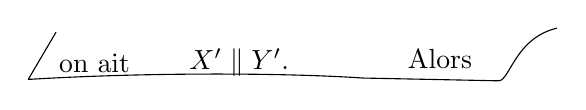
\begin{tikzpicture}[x=1em,y=1em,line cap=round,line join=round]
\node[anchor=west,inner sep=0pt] at (0,0) {\deleted{on ait}};
\node[anchor=west,inner sep=0pt] at (4.7,0) {\deleted{$X'\parallel Y'$.}};
\node[anchor=west,inner sep=0pt] at (12.6,.15) {\deleted{Alors}};
\draw (-.1,1.1)--(-1.1,-.6) .. controls (3,-.35) and (8,-.35) .. (11,-.55)--(15.9,-.65)
 .. controls (16.3,-.65) and (16.5,.9) .. (18,1.25);
\end{tikzpicture}}

On voudra la

\uline{Propriété 1} Soient $F,G\in\mathscr F$, $F\mathrel{\tikz[baseline=-.4ex,x=.65em,y=.65em]{\draw (0,1.1)--(1,.5)--(0,-.1) (1,1.1)--(0,.5)--(1,-.1);}}G$, $L=F\cap G$. Soient $F'\ll F,\ G'\ll G$. Alors
\[
\begin{aligned}
 & F'\mathrel{\tikz[baseline=-.4ex,x=.65em,y=.65em]{\draw (0,1.1)--(1,.5)--(0,-.1) (1,1.1)--(0,.5)--(1,-.1);}}G'\\
\Longleftrightarrow\quad & F'_{L}\mathrel{\tikz[baseline=-.4ex,x=.65em,y=.65em]{\draw (0,1.1)--(1,.5)--(0,-.1) (1,1.1)--(0,.5)--(1,-.1);}}G'_{L}
\end{aligned}
\]

cf \deleted{p.} GF $\underline{\overline{\mathrm{VI}}}$, p.~\uline{\unsure{73|13}} -- On a en tous cas tjrs $\mathrel{\tikz[x=.5em,y=.30em]{\draw (0,.12)--(1.2,.12) (.18,.45)--(1.16,.45); \draw (1.28,.68)..controls(1.5,.5)and(1.58,.05)..(1.56,-.25)..controls(1.45,-.3)and(1.27,-.3)..(1.1,-.3);}}$
\deleted{Montrons qu'on a bien en $\Rightarrow$. En effet,}

Ceci est équivalent (si on le voit de façon générale) à l'ancien At 12, qui prend le nom

% slanted
\margin{\uline{Critère} de \uline{compatibilité} pour les raffinements de \uline{sous-figures}\quad Mais c'est faux dans le cas simplicial, ex :}%
\figure{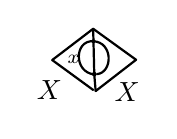
\begin{tikzpicture}[x=1em,y=1em,line cap=round,line join=round]
\draw[thick] (1.48,.04)--(0,1.12)--(1.48,2.25)--(3.03,1.13)--(1.57,0);
\draw[thick] (1.62,.61) .. controls (2.20,.68) and (2.20,1.76) .. (1.49,1.80)
 .. controls (.80,1.85) and (.76,.68) .. (1.52,.60);
\draw[thick] (1.48,2.25)--(1.52,.59)--(1.57,0);
\fill (1.49,1.80) circle (.074) (1.52,.61) circle (.085);
\node at (.77,1.16) {\scriptsize $x$};
\node at (-.10,.04) {$X$};
\node at (2.71,-.04) {$X$};
\end{tikzpicture}}
% slanted
\margin{Mais on aura $X'_{L}\parallel Y'_{L}\Longrightarrow X'\mathrel{\tikz[x=.55em,y=.60em,line cap=round]{\draw (0,-.12)--(0,1) (.48,-.12)--(.48,1) (-.06,.30)--(.54,.47) (-.05,.51)--(.53,.65);}}Y'$, C'est un \unsure{contre-exemple|contre-exple|contre exemple} à l' : At $\parallel$, et a fortiori à \deleted{\unsure{ex}} At 11 (cf GF $\underline{\overline{\mathrm{VI}}}$, p. 67,68)}%

% Oblique ancien sits above/right of Soient without a secure insertion caret. Its lexical reading is resolved; its intended grammatical attachment is not.
\uline{At DD} 1 \tikz[baseline=(s.base),x=1em,y=1em]{\node[anchor=west,inner sep=0pt] (s) at (0,0) {Soient}; \node[anchor=west,inner sep=0pt,rotate=47] at (4.2,.6) {\inserted{ancien}};} $X,Y\ \unsure{o|,}\ X',Y'\in M$, $X\mathrel{\tikz[baseline=-.4ex,x=.65em,y=.65em]{\draw (0,1.1)--(1,.5)--(0,-.1) (1,1.1)--(0,.5)--(1,-.1);}}Y,\ X'\ll X,Y'\ll Y$. \margin{\tikz[x=.5em,y=.5em]{\draw (0,0)--(0,4.25);}}Posons $K=X\cap Y=\underset{Z\in\widetilde X\cap\widetilde Y}{\mathrm{Sup}}\,Z$. Alors $X'_{L}\mathrel{\tikz[baseline=-.4ex,x=.65em,y=.65em]{\draw (0,1.1)--(1,.5)--(0,-.1) (1,1.1)--(0,.5)--(1,-.1);}}Y'_{L}$ implique $X'\mathrel{\tikz[baseline=-.4ex,x=.65em,y=.65em]{\draw (0,1.1)--(1,.5)--(0,-.1) (1,1.1)--(0,.5)--(1,-.1);}}Y'$ \quad (NB \unsure{l'inverse|l'énoncé} \deleted{\unsure{est}} est tjrs vrai)

% The following literal antecedents use C-prime, while the conclusions use G-prime; the discrepancy is not emended.
\uline{Corollaire} 1 \quad la ``propriété'' ci dessus

\[
F\parallel G,\ F'\ll F,\ C'\ll G\ \Longrightarrow\ F'\parallel G'
\tag*{\makebox[0pt][r]{\makebox[\displaywidth][l]{\uline{Corollaire} 2}}}
\]

Plus gén. \quad Si $F\mathrel{\tikz[baseline=-.4ex,x=.65em,y=.65em]{\draw (0,1.1)--(1,.5)--(0,-.1) (1,1.1)--(0,.5)--(1,-.1);}}G,\ F'\ll F,\ C'\ll G$, alors
\[
 F'\parallel G'\ \Longleftrightarrow\ F'_{L}\parallel G'_{L}
\]
